%   MSc Business Analytics Dissertation
%
%   Title:     Aaa Bbbbbbb Cccccccccc
%   Author(s): Xxxxxx Xxxxxxxxx and Yyy Yyyyyyyyy
%
%   Chapter 5: Results
%
%   Change Control:
%   When     Who   Ver  What
%   -------  ----  ---  --------------------------------------------------------------
%   11Feb11  AB    0.1  Begun 
%

\chapter{Results}\label{C.Results}

\section{Overview}
Model prediction accuracy of original test data set was 99.65\%, which is practically impossible. As discussed in chapter \ref{C.intro} actual data received from KPMG was made up using pre-defined formulas and rules to make it look real. Data didn't cover all possible scenario for a loan portfolio and achieving an accuracy of 99\% in credit scoring model is difficult as one needs to train model recursively with large data size covering all permutations and combinations of situations for loan default.


\section{Introduction}\label{S.intro5}

Original data set consist of 237389 observations and 35 variables, according to data 95\% loan applications will not default, and only 5\% application had chances to default. Therefore, to consider all possible scenarios data has been modified and a data subset has been generated from original dataset to carry experiments. New dataset has 36696 observations and 26 variabls. 

\section{Performance}
\textbf{Decision Tree over Logistic Regression:}

\cite{long1993comparison} studied decision tree application for classifying heart disease patient and compared the performance of decision tree with logistic regression. \cite{long1993comparison}, also noted that logistic regression model failed to consider missing data and decision tree model easily worked when data was noisy. \cite{satchidananda2006comparing}, build credit scoring model and found that decision tree produce a more precise model and good performance in comparison to logistic regression.

In this research work, decision tree performance did better against the logistic regression performance. Decision tree accuracy is 81.11\%, and logistic regression accuracy is 68.34\%. Based on the results of previous research work and after considering current experiments results on KPMG dataset, it is appropriate to build the business dashboard using decision tree model.

Another advantage of using decision tree model is that one can control the growth of decision tree using 'split' setting by doing so model performance can be optimised. On the other hand,  to train model with logistic regression, one to select the restricted number of independent variables, otherwise, the model can not be trained with many variables as vector size response variable grows exponentially.

Significant Variables in Logistic regression:
\begin{verbatim}
[1] "CreditRating"               "PropertyValue"             
 [3] "LoanBalance"                "LTV"                       
 [5] "NewLoanYes"                 "ProbationaryLoansYes"      
 [7] "MortgageTypeOwner Occupied" "CountyCavan"               
 [9] "CountyDonegal"              "CountyDublin"              

\end{verbatim}

\begin{table}[!htb]
\centering
\caption{Comparison of Logistic Regression and Decision Tree performance}
\label{table:results}
\begin{tabular}{@{}lccc@{}}
\toprule
\textbf{Model}               & \textbf{AUROC} & \textbf{KS} & \textbf{Gini} \\ \midrule
\textbf{Logistic Regression} & 68.34          & 13.53       & 36.68         \\
\textbf{Decision Tree}       & 81.11          & 60.04       & 62.22         \\ \bottomrule
\end{tabular}
\end{table}

In table. \ref{table:results}, KS is the Kolmogorov-Smirnov goodness-of-Fit Test (or KS-Test), GINI is Gini coefficient of inequality distribution of response variable and AUC is Area under ROC (Receiver Operating Chaterstics) curve.\\

\begin{figure*}[t!]
    \centering
    \begin{subfigure}
        \centering
        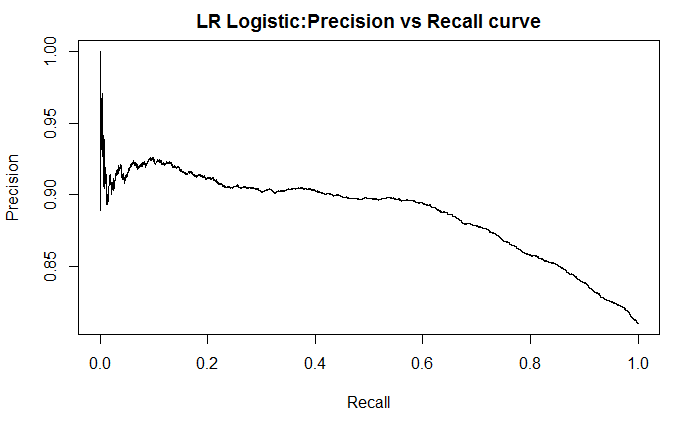
\includegraphics[height=1.2in]{LRrecall.png}
        \caption{Logistic Regression}
    \end{subfigure}%
    \begin{subfigure}
        \centering
        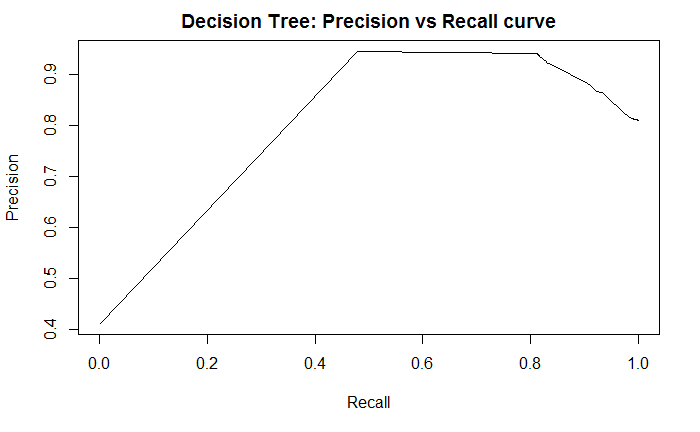
\includegraphics[height=1.2in]{DRrecall.png}
        \caption{Decision Tree}
    \end{subfigure}
    \caption{Precision vs Recall curve}
\end{figure*}


\begin{center}
\begin{figure}[!htb]
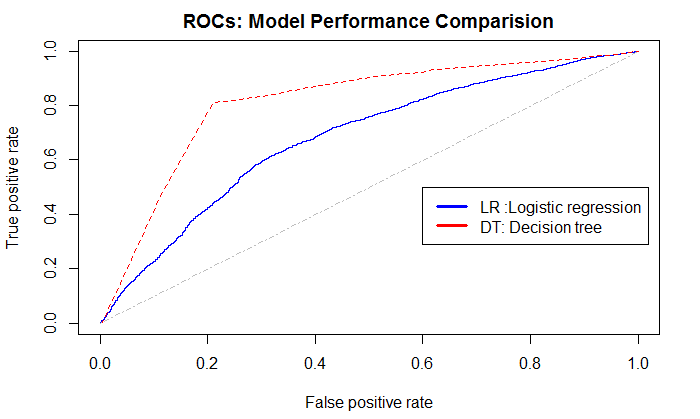
\includegraphics[width=\textwidth]{results1.png}
\centering
\caption{ROCs for logistic regression vs decision tree}{\textbf{Source:} Plotted in R Studio}
\label{fig:result}
\end{figure}
\end{center}

Receiver under curve is one of technique to estimate the performance of predictive model.
